\begin{comment}

\subsection{Дедекиндовы сечения. Определение действительных чисел по Дедекинду. Полнота $\R$ по Дедекинду.}

\subsubsection{Неполнота рациональных чисел.}
$r = \cfrac{p}{q},p\in \Z,q\in\N $\\
Дробь можно сделать несократимой.\\
Пусть $(\cfrac{p}{q})^2 = 2$ - несократимая дробь $\Rightarrow p^2 = 2q^2 \Rightarrow p = 2k$ (p - чётное число) \\
$k^2 = 2q^2 \Rightarrow q^2 = 2k^2 \Rightarrow $ q - чётное число
\\т.к. дробь несократимая, а числитель и знаменатель чётные, то она на самом деле сократимая. Противоречие! \\
Значит это число \textbf{нельзя} представить рациональной дробью.
\begin{figure}[h]
    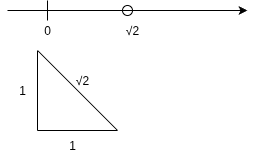
\includegraphics[width=0.2\linewidth]{images/Дедекиндовы сечения/Начало дедекиндовых сечений.png}
\end{figure}\\
Если на оси отметить все рациональные числа точками, то $\sqrt{2}$ - будет выколотой точкой.
\subsubsection*{Отрезки}
$I_n = [a_n, b_n] = \{ r \in \Q\; |\; a_n \leq r \leq b_n \}$, где $a_n, b_n \in \Q$
\begin{tcolorbox}
Будем считать, что $\forall n [a_{n+1}, b_{n+1}] \subset [a_n, b_n]$ - \textbf{вложенные отрезки.}\\
Это значит, что $a_n \leq a_{n+1} \leq b_{n+1} \leq b_n$ и следующий отрезок меньше предыдущего.
\end{tcolorbox}
\begin{tcolorbox}
    $b_n - a_n \xrightarrow{n\to\infty} 0$ - \textbf{стягивающиеся отрезки.}
\end{tcolorbox}
\textbf{Дальше будем подразумеваться}, что все последовательности $\{I_n\}$ - вложенные и стягивающиеся в точку.
\begin{figure}[h]
    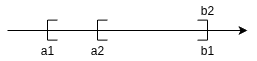
\includegraphics[width=0.25\linewidth]{images/Дедекиндовы сечения/Смысл отрезков.png}
\end{figure}\\
Что нам дают такие отрезки: $\forall r$ \\
\begin{equation}
    \exists n: r < a_n \Rightarrow \forall m > n:\; r < a_m
\end{equation}
\begin{equation}
    \exists n: r > b_n \Rightarrow \forall m > n:\; r > b_m
\end{equation}
\begin{equation}
    \forall n: a_n \leq r \leq b_n
\end{equation}
\begin{enumerate}
    \item левый класс для $\{I_n\}$ (всегда не пуст)
    \item правый класс для $\{I_n\}$ (всегда не пуст)
    \item центральный класс для $\{I_n\}$ (может быть пустым учитывая $r \in \Q)$. Не может содержать более 1 Q числа.
\end{enumerate}
Слово "класс" подразумевает множество.
\begin{tcolorbox}
    \textbf{Дедекиндово сечение}  - множество рациональных чисел (Q) порождённое последовательностью $\{I_n\}$.
\end{tcolorbox}
Тогда каждому действительному числу будет соответствовать своё дедекиндово сечение.

\begin{tcolorbox}
\textbf{Определение}\\
\textit{$\{I_n\}$ и $\{I_n``\}$ - \textbf{эквиваленты}, если они порождают одинаковые разбиения на классы}
\end{tcolorbox}

\begin{tcolorbox}
\textbf{Теорема 1}\\
$\{ I_n \}\sim$ эквивалентна $\{ I_n` \} \Leftrightarrow$
\begin{enumerate}
    \item $\forall n \;\; a_n - a_n` \xrightarrow{n \to \infty} 0 $\\
    ИЛИ
    \item $\forall n a_n \leq b_n`,\; a_n` \leq b_n$
\end{enumerate}
\end{tcolorbox}

\begin{tcolorbox}[title=Доказательство Т1, breakable]
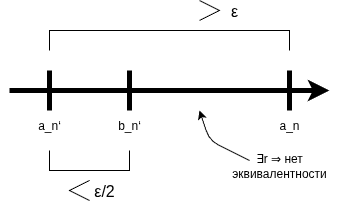
\includegraphics[width=0.4\linewidth]{images/Дедекиндовы сечения/Доказательство Т1.png}\\
\textbf{Только п.1.} \\
$\Rightarrow$: $\{ I_n \} \sim \{ I_n` \} \Rightarrow a_n-a_n` \rightarrow 0$\\
от противного: тогда $a_n-a_n` \nrightarrow 0 \Leftrightarrow \\ 
\exists \eps>0:\; \forall N\;\; \exists n > N\; |a_n - a_n`| \geq \eps $ \\
$\Rightarrow $ для бесконечно многих номеров либо $a_n-a_n` > \eps$, либо $a_n` - a_n > \eps$\\
Пусть для бесконечно многих номеров $a_n - a_n` > \eps$ \\
$\exists n_\eps$ длина $[a_n`, b_n`] < \cfrac{\eps}{2}$\\
$b_n`-a_n` \rightarrow 0 \; \exists n_\eps: \; \forall n > n_\eps\; |b_n`-a_n`| < \cfrac{\eps}{2}$\\
Т.к. $\exists r \in [b_n`, a_n]$, то она принадлежит правому классу $\{I_n`\}$ и левому классу $\{I_n\}$. Последовательности не эквивалентны.\\

$\Leftarrow: a_n - a_n`\; \xrightarrow{n\rightarrow \infty} 0 \Rightarrow \{ I_n \} \sim \{ I_n` \}$\\
От противного: пусть $\{ I_n \} \nsim \{ I_n` \}$, то есть $\exists r \in Q\; r$ из левого класса для одной и центрального или правого класса другой.

r из левого класса $\{ I_n \} \exists n: r < a_n$
\begin{enumerate}
    \item[i.] r из правого класса $\{ I_n` \} \Rightarrow \exists n`: \forall n > n`\;\; a_n` \leq b_n` < r < a_n \leq a_m$\\
    \item[ii.] r из центрального класса $\{ I_n` \}$\\
    $\exists n: r < a_n$ Пусть $\eps = a_n - r(>0)$\\
    $\exists n_\eps: \forall m > n_\eps |b_m`-a_m`| < \cfrac{\eps}{2} \Rightarrow [a_m`,b_m`]$ на расстоянии не меньше $\cfrac{\eps}{2}$ от $a_n$
\end{enumerate}

\textbf{2 вариант доказательства в обратную сторону.}\\
$\Leftarrow: a_n - a_n`\; \xrightarrow{n\rightarrow \infty} 0 \Rightarrow \{ I_n \} \sim \{ I_n` \}$\\
а) совпадение левых классов $r \in $ левый класс для $\{I_n\}$
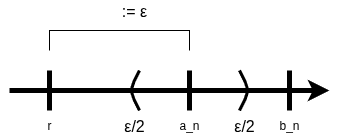
\includegraphics[width=0.4\linewidth]{images/Дедекиндовы сечения/Доказательство Т1.2.png}\\
$\exists n: r < a_n$\\
$\exists n_\eps: \forall n>n_\eps \;\;|a_n-a_n`| < \cfrac{\eps}{2} \Rightarrow r < a_n` \Rightarrow r\ \in $ левый класс для $\{I_n`\}$ \\
б) правые классы аналогично
\end{tcolorbox}

\subsubsection{Ограничение на количество элементов центрального класса.}
Если r из центрального класса, то $\forall n: \; a_n \leq r \leq b_n$\\
А если $\exists r`,r \in $ центральный класс $r<r`$, то $a_n \leq r < r` \leq b_n$. Тогда длина отрезка не может быть меньше длины отрезка $[r,r`]$ значит она не стремится к 0.\\
В центральном классе может быть либо 1 число либо 0.
\subsubsection*{Пример 2-х последовательностей стягивающихся к 0}
$\{I_n\} = [\cfrac{1}{2n},\cfrac{1}{2n}]\;\; \{I_n`\} = [\cfrac{1}{2n+1},\cfrac{1}{2n+1}] \;\; \{I_n``\} = [0,\cfrac{1}{2n+1}]$ Они определяют 1 и то же число.
\subsubsection*{Пример 2-х последовательностей стягивающихся к $\sqrt{2}$}
$[\sqrt{2} - \cfrac{1}{n}, \sqrt{2} + \cfrac{1}{n}]$
\subsubsection{Действительные числа}
\begin{tcolorbox}
\textit{\textbf{Действительные числа} - это вложенные стягивающиеся отрезки с рациональными концами. Числа равны, если последовательность $\{I_n\} \sim \{I_n`\}$  }\\
\textit{\textbf{Действительные число} - отождествляется с дедекиндовым сечением, порождённым $\{[a_n, b_n]\}$ . Числа равны, если последовательность $\{[a_n, b_n]\} \sim \{[a_n`, b_n`]\}$  }
\end{tcolorbox}

\subsubsection*{Ограничение на количество элементов центрального класса.}
Если r из центрального класса, то $\forall n: \; a_n \leq r \leq b_n$\\
А если $\exists r`,r \in $ центральный класс $r<r`$, то $a_n \leq r < r` \leq b_n$. Тогда длина отрезка не может быть меньше длины отрезка $[r,r`]$ значит она не стремится к 0.\\
В центральном классе может быть либо ё число либо 0.
\subsubsection*{Пример 2-х последовательностей стягивающихся к 0}
$\{I_n\} = [\cfrac{1}{2n},\cfrac{1}{2n}]\;\; \{I_n`\} = [\cfrac{1}{2n+1},\cfrac{1}{2n+1}] \;\; \{I_n``\} = [0,\cfrac{1}{2n+1}]$ Они определяют 1 и то же число.
\subsubsection*{Пример 2-х последовательностей стягивающихся к $\sqrt{2}$}
$[\sqrt{2} - \cfrac{1}{n}, \sqrt{2} + \cfrac{1}{n}]$

\subsubsection{Полнота по Дедекинду}
\textbf{Полнота по Дедекинду} - это непустота центрального класса. 


\subsection{Лемма об отделимости}

\subsubsection{Отделимость множеств}
Пусть $A, B \subset \mathbb{R}$, $A \neq \varnothing, B \neq \varnothing$, и выполнено условие:
\[ \forall a \in A, \forall b \in B \implies a \leq b \]

\begin{center}
    % Здесь должна быть ваша картинка
    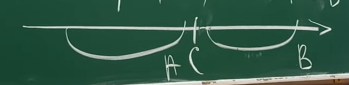
\includegraphics[width=0.5\linewidth]{II/images/Отделимость}
\end{center}

\textbf{Утверждение:}
\[ \exists c \in \mathbb{R}: \quad \forall a \in A, \forall b \in B \implies a \leq c \leq b \]
Такое число $c$ называется \textit{разделяющим} числом.

\begin{tcolorbox}[title=Доказательство]
    Рассмотрим два случая взаимного расположения множеств:

    \begin{enumerate}
        \item \textbf{Случай 1:} $A \cap B \neq \varnothing$.
        
        Это значит, что существует элемент $c \in A \cap B$.
        \[
        \begin{cases}
            c \in A \Rightarrow \forall b \in B \;\; c \leq b \quad \text{(по условию леммы)} \\
            c \in B \Rightarrow \forall a \in A \;\; a \leq c \quad \text{(по условию леммы)}
        \end{cases}
        \]
        Объединяя неравенства, получаем:
        \[ \forall a \in A, \forall b \in B \implies a \leq c \leq b \]
        \textit{Замечание:} В этом случае разделяющее число единственно (если бы существовало $c' \neq c$, это привело бы к противоречию с условием $a \le b$ для элементов пересечения).

        \item \textbf{Случай 2:} $A \cap B = \varnothing$.
        
        Тогда $\forall a \in A, \forall b \in B \implies a < b$ (равенство невозможно, так как пересечение пусто).
        
        Расширим множества до полного покрытия прямой $\mathbb{R}$ (построение сечения Дедекинда).
        
        \begin{center}
            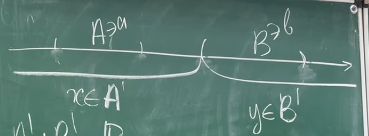
\includegraphics[width=0.5\linewidth]{II/images/Отделимость2}
        \end{center}
        
        Определим множество $B'$ (все точки правее $B$ + само $B$):
        \[ B' := \{ y \in \mathbb{R} \mid \exists b \in B: b \leq y \} \]
        Свойства $B'$:
        \begin{itemize}
            \item $B \subset B'$ (так как $b \le b$).
            \item $A \cap B' = \varnothing$. (Действительно, если $a \in A$, то $\forall b \in B: a < b$, значит, $a$ не может быть больше или равно никакому $b$).
        \end{itemize}
        
        Определим множество $A'$ как дополнение:
        \[ A' := \mathbb{R} \setminus B' \]
        Так как $A \cap B' = \varnothing$, то $A \subset A'$. Значит, $A' \neq \varnothing$ и $B' \neq \varnothing$.
        
        Имеем разбиение прямой: $A' \cup B' = \mathbb{R}$, $A' \cap B' = \varnothing$.
        
        Докажем, что любой элемент из $A'$ меньше любого элемента из $B'$:
        \[ \forall x \in A', \forall y \in B' \implies x < y \]
        (Доказательство от противного: если $x \ge y$ и $y \in B'$, то по определению $B'$ существует $b \in B$, такое что $b \le y \le x$. Но если $x \ge b$, то $x$ должен лежать в $B'$, а он в $A'$).
        
        \textbf{Построение разделяющей точки (Метод вложенных отрезков):}
        
        Возьмем произвольные $a_1 \in A'$ и $b_1 \in B'$.
        
        \begin{center}
            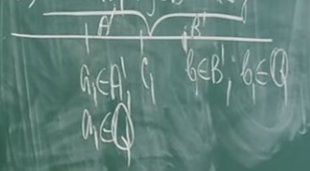
\includegraphics[width=0.5\linewidth]{II/images/Отделимость3}
        \end{center}
        
        1. Найдем середину: $c_1 = \frac{a_1 + b_1}{2}$.
        \begin{itemize}
            \item Если $c_1 \in A'$, то новый отрезок $[a_2, b_2] := [c_1, b_1]$.
            \item Если $c_1 \in B'$, то новый отрезок $[a_2, b_2] := [a_1, c_1]$.
        \end{itemize}
        Получили $[a_2, b_2] \subset [a_1, b_1]$, причем $a_2 \in A', b_2 \in B'$.
        Длина отрезка: $|b_2 - a_2| = \frac{1}{2} |b_1 - a_1|$.
        
        2. Повторяем процесс $n$ раз. Получаем систему вложенных отрезков:
        \[ [a_1, b_1] \supset [a_2, b_2] \supset \dots \supset [a_n, b_n] \supset \dots \]
        Где $\forall n: a_n \in A', b_n \in B'$.
        Длина отрезка стремится к нулю:
        \[ |b_n - a_n| = \frac{1}{2^{n-1}} |b_1 - a_1| \xrightarrow[n\to \infty]{} 0 \]
        
        3. По принципу вложенных отрезков (Коши-Кантора) существует единственная общая точка $c$:
        \[ \exists! c \in \mathbb{R}: \quad c = \bigcap_{n=1}^{\infty} [a_n, b_n] \]
        
        Для этой точки выполняется:
        \[ \forall n \;\; a_n \leq c \leq b_n \]
        Следовательно, $c$ разделяет множества $A'$ и $B'$:
        \[ \forall x \in A', \forall y \in B' \implies x \leq c \leq y \]
        
        \begin{center}
            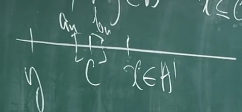
\includegraphics[width=0.5\linewidth]{II/images/Отделимость4}
        \end{center}
        
        Так как $A \subset A'$ и $B \subset B'$, то $c$ разделяет и исходные множества:
        \[ \forall a \in A, \forall b \in B \implies a \leq c \leq b \]
    \end{enumerate}
\end{tcolorbox}

\subsubsection{Существование точной грани}
Из леммы об отделимости следует существование точной верхней и нижней грани множества.

\textbf{Следствие 1.} Если множество $E \subset \mathbb{R}$ ограничено сверху ($E \neq \varnothing$), то существует точная верхняя грань (супремум):
\[ \exists M \in \mathbb{R}: M = \sup E \]

\textbf{Следствие 2.} Если множество $E \subset \mathbb{R}$ ограничено снизу ($E \neq \varnothing$), то существует точная нижняя грань (инфимум):
\[ \exists m \in \mathbb{R}: m = \inf E \]

\begin{tcolorbox}[title=Доказательство (для супремума)]
    Пусть $E$ ограничено сверху.
    Обозначим $M_{set}$ — множество всех верхних граней множества $E$.
    Так как $E$ ограничено сверху, $M_{set} \neq \varnothing$.
    Так как $E \neq \varnothing$, то $E$ не пусто.
    
    По определению верхней грани:
    \[ \forall x \in E, \forall m \in M_{set} \implies x \leq m \]
    
    Применим лемму об отделимости к множествам $A = E$ и $B = M_{set}$.
    Существует число $c \in \mathbb{R}$, такое что:
    \[ \forall x \in E, \forall m \in M_{set} \implies x \leq c \leq m \]
    
    1. Так как $\forall x \in E, x \leq c$, то $c$ является верхней гранью $E$. Значит $c \in M_{set}$.
    2. Так как $\forall m \in M_{set}, c \leq m$, то $c$ является наименьшей из верхних граней.
    
    Следовательно, $c = \sup E$.
\end{tcolorbox}



\subsection{Лемма об отделимости.}
\subsubsection{Отделимость множеств}
\[ A, B \subset \R, A, B \not= \varnothing,\; \forall a \in A, \forall b \in B \]
\begin{center}
	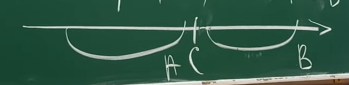
\includegraphics[width=0.5\linewidth]{II/images/Отделимость}
\end{center}
\[ a \leq b \Rightarrow \exists c \in \R: \]
\[ \forall a \in A, \forall b \in B \;\; a \leq c \leq b \]

\begin{tcolorbox}[title=Доказательство]
	\begin{enumerate}
		\item $ A \cap B \not= \varnothing \;\; \exists c \in Aa \cap B $
	\[ 
	\begin{cases}
		c \in A \Rightarrow \forall b \in B \;\; c \leq b\\
		c \in B \Rightarrow \forall a \in A \;\; a \leq c
	\end{cases} \Rightarrow \forall a \in A \; \forall b \in B \;\; a \leq c \leq b
	\]
	Как доп вопрос может спросить про единственность $c$.

	\item $ A\cap B = \varnothing\; \forall a \in A, \forall b \in B $
		$a \leq b$, если бы $a=b \in A\cap B \Rightarrow a < b$ 

Пусть множется A и B непустые.
\begin{center}
	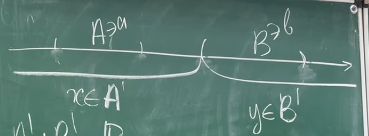
\includegraphics[width=0.5\linewidth]{II/images/Отделимость2}
\end{center}
\[ B` := \{ y \in \R:\; \exists b \in B: b \leq y \} \]
\[ \forall b \in B \;\; b \leq b \Rightarrow b \in B` \]
\[ \forall a \in A \; \forall b \in B\;\; a < b \Rightarrow a \not\in B` \Rightarrow A\cap B =\varnothing \]
\[ A` := \R \setminus B` \supset A \Rightarrow A` \not= \varnothing \]
\[ A` \cup B` = \R \]
\[ \forall y \in B` \Rightarrow \exists b \in B: b \leq y \]
\[ \forall x \in A` \;\; \forall b \in B \;\; x \leq b \]
Если бы не так, то $\exists b \in B: x \geq b \Rightarrow x \in B` \Rightarrow x \in A`$
\[ \forall x \in A` \; \forall y \in B` \; \exists b_y: x < b_y \leq y \]
Свойства:
\begin{enumerate}
	\item $A`,B` \not= \varnothing$
	\item $A` + B` = \R$ 
	\item $\forall x \in A`, \forall y \in B` \;\; x < y$
\end{enumerate}
\begin{center}
	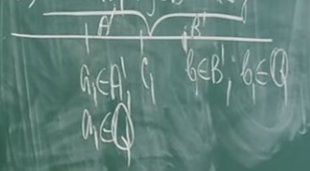
\includegraphics[width=0.5\linewidth]{II/images/Отделимость3}
\end{center}
\[ c_1 = \frac{a_1 + b_1}{2} \]
\[ c_1 \in \Q \]
Если $c_1 \ in A`$, то 
\[ [a_2, b_2] := [c_1, b_1] \]
Если $c_1 \in B`$, то $[a_2, b_2] := [a_1, c_1]$
\[ [a_2, b_2] \supset [a_1, b_1] \]
Длинна $[a_2, b_2] = \frac{1}{2}$ длинны $[a_1, b_1]$
\[ c_2 = \frac{a_2 + b_2}{2} \]
$[a_3, b_3]$ тот из отрезков $[a_2, c_2]$ и $[c_2, b_2]$, концы которого $a_3 \in A`$ \; $b_3 \in B`$\\ 
... \\ 
$[a_n, b_n]$ длиинна $[a_m, b_n] = \frac{1}{2}$ длинна $[a_{n-1}, b_{n-1}] = \frac{1}{2^{n-1}}$ длина $[a_1, b_1] \xrightarrow[n\to \infty]{} 0$ 
\[ \forall a_n \in A`, \forall b_n \in B` \Rightarrow \exists c \in \R \; \forall n \; c \in [a_n, b_n]\]
\[ \forall n\;\; a_n \leq c \leq b_n \]
\[ \forall x \in A`, \forall y \in B` \;\; x\leq c \leq y \]
\begin{center}
	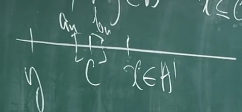
\includegraphics[width=0.5\linewidth]{II/images/Отделимость4}
\end{center}
C разделяет A` и B` $\Rightarrow$ разделяет A и B. 

	\end{enumerate}
\end{tcolorbox}


Из отделимости следует существование точной верхней грани. 


\textbf{Следствие.} Если E ограничено сверху, то существует точная верхняя грань E. 
\[ M = \sup E \]
\textbf{Следствие.} Если E ограничено снизу, то существует точная нижняя грань E. 
\[ m = \inf E \]
\begin{tcolorbox}[title=Доказательство]
	E ограничено сверху, M - множество верхних граней. $\forall x \in E, \forall m \in M$
	\[ x \leq m \Rightarrow \exists m` \in \R \]
	\[ \forall x \in E, \forall m \in M \;\; x \leq m` \leq m \]
\end{tcolorbox}
\subsection{Точная верхняя и нижняя грани ограниченных множеств из В. Теорема Вейерштрасса о существовании точной верхней грани ограниченного сверху множества как следствие леммы об отделимости (принцип полноты В по Вейерштрассу).}

\subsubsection{Точная верхняя грань}
\[ E \subset \R, E \not=  \varnothing \]
\begin{tcolorbox}
	\textbf{Определение.} E ограничено сверху, если $\exists M \in \R, \forall x \in E: x \leq M$


	M - Верхняя грань (граница)
\end{tcolorbox}
Ограниченность снизу анологична.
\begin{tcolorbox}
	\textbf{Определение.} M - точная верхняя грань E, если 
	\begin{enumerate}
		\item M - верхняя граница E 
		\item M - наименьшая верхняя граница, т.е. $\forall M` < M\; \exists x_M \in E: x_M > M`$
			
	\end{enumerate}
\end{tcolorbox}

\subsubsection{Полнота по Вейерштрассу}
\begin{tcolorbox}
    \textbf{Принцип полноты множества по Вейерштрассу}
    Принцип полноты множества по Вейерштрассу означает, что любое ограниченное сверху множество имеет точную верхнюю грань     
\end{tcolorbox}

\begin{tcolorbox}
    \textbf{Определение}
    $\{a_n\}$ монотонна, если возрастает/ строго возрастает/убывает/строго убывает.
\end{tcolorbox}

\begin{tcolorbox}
    \textbf{Теорема по Вейерштрассу}
    \begin{enumerate}
        \item $\{a_n\} \uparrow \; \Rightarrow a_n \to sup\{ a_n \}$
        \item $\{a_n\} \downarrow \; \Rightarrow a_n \to inf\{ a_n \}$
    \end{enumerate}
\end{tcolorbox}

\begin{tcolorbox}
    \textbf{Определение}
    $sup \{a_n\}$ - это $sup$ множества членов последовательности.
\end{tcolorbox}

\begin{tcolorbox}[title=Доказательство полноты $\R$ по Вейерштрассу]
    \textbf{Доказательство}
    \begin{enumerate}
        \item Ограничено сверху $\exists M: \forall n a_n \leq M \Rightarrow \exists sup\{a_n\} = M \in \R$\\
        По определению предела $\forall \varepsilon > 0 \exists n_\varepsilon: \forall n > n_\varepsilon |a_n - M| < \varepsilon $\\
        $\Leftrightarrow M-\varepsilon<a_n<M+\varepsilon$ т.к. $M=sup\{a_n\}$, то $a_n \leq M$ надо проверить $M-\varepsilon<a_n\leq M$\\
        M - наименьшая верхняя грань $\Rightarrow \exists n_\varepsilon: \forall n > n_\varepsilon \;\;\;\;\; M-\varepsilon \leq a_{n_\varepsilon} \leq a_n \leq M $\\
        т.е. по определению 
        \[M = \lim_{n\to\infty} a_n\]
        \textbf{Следствие} $\{a_n\}$ - монотонна $\{a_n\}$ - сходится $\Leftrightarrow \{a_n\}$ - ограничена.
    \end{enumerate}
\end{tcolorbox}


\subsection{Последовательности стягивающихся отрезков с действительными концами. Теорема Кантора о стягивающихся отрезках с действительными концами (принцип полноты ® по Кантору).}
\subsubsection{Принцип вложенных отрезков (полнота $\R$ по Кантору)}
\[ \forall n \; A_n \not= \varnothing \]
\begin{enumerate}
	\item $A_1 \subset A_2 \subset A_3 \subset ... \subset A_k $\\
		\[\cap_{n=1} A_n \not= \varnothing\]
	\item $A_1 \subset A_2 \subset A_3 \subset ... \subset A_n \subset A_{n+1} \subset ... $\\
		\begin{enumerate}
			\item $A_k := \{ x \in \R,\; x \geq k \}$\\
				\[ \cap_{k=1}^{\infty} A_k \not= \varnothing \]
			\item $A_k = (0, \frac{1}{k}]$
				\begin{center}
					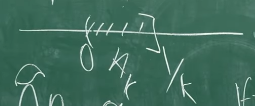
\includegraphics[width=0.5\linewidth]{II/images/Кантор}
				\end{center}
				\[ \cap_{k=1}^{\infty} A_k = \varnothing \]
				\[ \forall k \; x \not\in A_k \]
			\item $A_k := (-\frac{1}{k};\frac{1}{k})$
				\[ \cap_{k=1}^{\infty} A_k = 0 \]
		\end{enumerate}
\end{enumerate}
\textbf{Теорема.} $ [a_1, b_1] \supset [a_2, b_2] \supset ... \supset [a_n, b_n] \supset [a_{n+1}, b_{n+1}] \supset ... $

\subsection{Полнота $\R$ по Дедекинду как следствие принципа стягивающихся отрезков.}

\subsection{Счётность множества, рациональных чисел и несчётность множества действительных чисел.}

\end{comment}

% \section{Действительные чсла. Числовые множества}
\subsection{Дедекиндовы сечения. Определение действительных чисел по Дедекинду. Полнота $\mathbb{R}$ по Дедекинду}

\textbf{Контекст:} Рассматривается проблема того, что $\sqrt{2} \notin \mathbb{Q}$. Вводятся вложенные отрезки с рациональными концами $I_n = [a_n, b_n]$, где $a_i, b_i \in \mathbb{Q}$.

Последовательность вложенных стягивающихся отрезков $\{[a_n, b_n]\}$ обладает свойствами:
\begin{enumerate}
    \item $[a_1, b_1] \supset [a_2, b_2] \supset \dots \supset [a_n, b_n] \supset [a_{n+1}, b_{n+1}]$;
    \item Длина отрезка $b_n - a_n \xrightarrow[n\to\infty]{} 0$.
\end{enumerate}

\subsubsection*{Дедекиндово сечение}
Для любого рационального числа $r \in \mathbb{Q}$ возможны три ситуации относительно последовательности $\{I_n\}$:
\begin{enumerate}
    \item $\exists n': r < a_{n'} \Rightarrow \forall m \ge n' \;\; r < a_m$ (число левее всех отрезков, начиная с некоторого).
    \item $\forall n \;\; a_n \le r \le b_n$ (число внутри всех отрезков).
    \item $\exists n'': r > b_{n''} \Rightarrow \forall m \ge n'' \;\; r > b_m$ (число правее всех отрезков, начиная с некоторого).
\end{enumerate}

\textbf{Определения. }
    \begin{itemize}
        \item Множество всех $r \in \mathbb{Q}$, для которых выполнено условие (1) — \textbf{левый класс} для $\{I_n\}$.
        \item Если существует $r \in \mathbb{Q}$, для которого выполнено условие (2) — это \textbf{центральный класс} для $\{I_n\}$ (может быть пустым).
        \item Множество всех $r$, для которых выполнено условие (3) — \textbf{правый класс} для $\{I_n\}$.
    \end{itemize}
    Такое разделение множества $\mathbb{Q}$ на классы называется \textbf{дедекиндовым сечением $\mathbb{Q}$, порожденным $\{I_n\}$}.

\subsubsection*{Определение действительного числа}
\textbf{Теорема. }
    Последовательности $\{I_n\}$ и $\{I'_n\}$ называются \textbf{эквивалентными} ($\{I_n\} \sim \{I'_n\}$), если они порождают одинаковые разбиения на классы.

\begin{tcolorbox}
    $\{I_n\} \sim \{I'_n\}$ тогда и только тогда, когда:
    \begin{enumerate}
        \item $\forall n \;\; a_n - a'_n \to 0$ при $n \to \infty$ (или $b_n - b'_n \to 0$).
        \item Или $\forall n \;\; a_n \le b'_n, \; a'_n \le b_n$ (пересечение непусто).
    \end{enumerate}
\end{tcolorbox}

\begin{tcolorbox}[title=Доказательство Теоремы, breakable]
    \textbf{1. Необходимость ($\Rightarrow$)}
    
    Дано: $\{ I_n \} \sim \{ I_n' \}$. Докажем, что $a_n - a'_n \to 0$.
    
    \textit{От противного.} Предположим, что $a_n - a'_n \nrightarrow 0$.
    Это означает, что существует $\varepsilon > 0$, такое что для бесконечного множества номеров $n$ выполняется:
    \[ |a_n - a'_n| \ge \varepsilon \]
    Пусть (для определенности) $a_n - a'_n \ge \varepsilon$, то есть $a_n \ge a'_n + \varepsilon$.
    
    Так как отрезки стягиваются ($|I'_n| \to 0$), начиная с некоторого номера $N$ длина отрезка $I'_n$ станет меньше $\varepsilon/2$:
    \[ b'_n - a'_n < \frac{\varepsilon}{2} \implies b'_n < a'_n + \frac{\varepsilon}{2}. \]
    
    Тогда получаем неравенство:
    \[ b'_n < a'_n + \frac{\varepsilon}{2} < a_n. \]
    Между числами $b'_n$ и $a_n$ (интервал ненулевой длины) всегда найдется рациональное число $r$:
    \[ b'_n < r < a_n. \]
    
    Анализируем число $r$:
    \begin{itemize}
        \item $r > b'_n \implies r$ принадлежит \textbf{правому} классу для $\{I'_n\}$.
        \item $r < a_n \implies r$ принадлежит \textbf{левому} классу для $\{I_n\}$.
    \end{itemize}
    Это противоречит условию эквивалентности (классы должны совпадать).
    Следовательно, предположение неверно, и $a_n - a'_n \to 0$.

    \medskip

    \textbf{2. Достаточность ($\Leftarrow$)}
    
    Дано: $a_n - a'_n \to 0$. Докажем, что $\{ I_n \} \sim \{ I_n' \}$.
    Достаточно показать, что совпадают их левые классы.
    
    Пусть $r$ — произвольное число из левого класса $\{I_n\}$.
    Это значит, что $\exists n_0: r < a_{n_0}$.
    Пусть $\delta = a_{n_0} - r > 0$.
    
    Так как $a_n - a'_n \to 0$, то начиная с некоторого номера $N$:
    \[ |a_n - a'_n| < \frac{\delta}{2}. \]
    В частности, $a'_n > a_n - \frac{\delta}{2}$.
    
    Тогда для достаточно больших $n$:
    \[ a'_n > a_{n_0} - \frac{\delta}{2} = (r + \delta) - \frac{\delta}{2} = r + \frac{\delta}{2} > r. \]
    
    Получили $r < a'_n$. Это означает, что $r$ принадлежит левому классу $\{I'_n\}$.
    
    Аналогично доказывается в обратную сторону.
    Левые классы совпадают $\implies$ последовательности эквивалентны.
\end{tcolorbox}

\begin{tcolorbox}[title=Доказательство Теоремы 1 (Пункт 2), breakable]
    \textbf{Условие:} $\{ I_n \} \sim \{ I_n' \} \iff \forall n \;\; (a_n \le b'_n \land a'_n \le b_n)$.
    
    \medskip
    \textbf{1. Необходимость ($\Rightarrow$)}
    
    Дано: $\{ I_n \} \sim \{ I_n' \}$. Докажем, что $a_n \le b'_n$ (второе неравенство аналогично).
    
    \textit{От противного.} Пусть $\exists n_0$, для которого $a_{n_0} > b'_{n_0}$.
    Тогда между числами $b'_{n_0}$ и $a_{n_0}$ существует рациональное число $r$:
    \[ b'_{n_0} < r < a_{n_0}. \]
    
    Исследуем принадлежность $r$:
    \begin{itemize}
        \item $r < a_{n_0} \implies r$ принадлежит \textbf{левому} классу для $\{I_n\}$.
        \item $r > b'_{n_0} \implies r$ принадлежит \textbf{правому} классу для $\{I'_n\}$.
    \end{itemize}
    
    Получили противоречие: если последовательности эквивалентны, их разбиения на классы должны совпадать. Число $r$ не может быть в левом классе одной и в правом классе другой.
    Следовательно, $a_n \le b'_n$.

    \medskip
    \textbf{2. Достаточность ($\Leftarrow$)}
    
    Дано: $\forall n \;\; a_n \le b'_n$ и $a'_n \le b_n$.
    Докажем, что $\lim_{n \to \infty} (a_n - a'_n) = 0$ (что по п.1 равносильно эквивалентности).
    
    Рассмотрим разность $a_n - a'_n$. Возможны два случая:
    
    \begin{itemize}
        \item Если $a_n \ge a'_n$, то пользуемся условием $a_n \le b'_n$:
        \[ 0 \le a_n - a'_n \le b'_n - a'_n. \]
        Так как длина отрезка $b'_n - a'_n \to 0$, то по теореме о зажатой последовательности $a_n - a'_n \to 0$.
        
        \item Если $a_n < a'_n$, то пользуемся условием $a'_n \le b_n$:
        \[ 0 \le a'_n - a_n \le b_n - a_n. \]
        Так как $b_n - a_n \to 0$, то $a'_n - a_n \to 0$.
    \end{itemize}
    
    В обоих случаях $|a_n - a'_n| \to 0$.
    Следовательно, $\{ I_n \} \sim \{ I_n' \}$.
\end{tcolorbox}

\textbf{Вывод:} Действительные числа определяются как классы эквивалентности вложенных стягивающихся отрезков с рациональными концами.

\textbf{Действительное число} отождествляется с дедекиндовым сечением, порождённым последовательность вложенных стягивающихся отрезков $\{[a_n, b_n]\}$, если $\{[a_n,b_n]\} ~ \{[a_n`, b_n`]\}$

\subsubsection*{5. Примеры}

\textbf{Пример 1: Число 0.}
\begin{itemize}
    \item $\{I_n\} = [-\frac{1}{n}, \frac{1}{n}]$
    \item $\{I_n'\} = [0, \frac{1}{n}]$
    \item $\{I_n''\} = [-\frac{1}{2^n}, \frac{1}{n^2}]$
\end{itemize}
У всех этих последовательностей центральный класс содержит число $0$. Все левые концы стремятся к 0. Они эквивалентны.

\textbf{Пример 2: Число $\sqrt{2}$.}
Рассмотрим приближения с недостатком и избытком:
$$ I_n = \left[ q_n, q_n + \frac{1}{n} \right], \quad \text{где } q_n^2 < 2 < (q_n + 1/n)^2 $$
Центральный класс такой последовательности пуст (в $\Q$ нет числа, квадрат которого равен 2), но последовательность определяет действительное число $\sqrt{2}$.

\subsubsection*{6. Полнота $\mathbb{R}$ по Дедекинду}

\begin{tcolorbox}
\textbf{Полнота по Дедекинду} означает, что для любой системы вложенных стягивающихся отрезков \textit{действительных} чисел существует (и единственна) общая точка.
\end{tcolorbox}

В контексте определения через рациональные отрезки:
Множество $\R$, построенное как совокупность классов эквивалентных последовательностей, является полным. То есть, если мы построим сечение уже над множеством $\R$, центральный класс никогда не будет пустым.


\newpage

\subsection{Лемма об отделимости}

\begin{definition}[Отделимость]
    Множество $C$ отделяет $A$ от $B$, если $\forall a \in A, \forall b \in B \implies a \le c \le b$.
\end{definition}

\begin{lemma}[Об отделимости]
    Пусть $A, B \subset \mathbb{R}$, $A \neq \varnothing, B \neq \varnothing$.
    Пусть выполнено условие: $\forall a \in A, \forall b \in B \implies a \le b$.
    
    Тогда $\exists c \in \mathbb{R}$, такое что $\forall a \in A, \forall b \in B \implies a \le c \le b$.
\end{lemma}

\begin{proof}
    Рассмотрим два случая:
    
    \textbf{Случай 1:} $A \cap B \neq \varnothing$.
    Тогда существует $c \in A \cap B$.
    \begin{itemize}
        \item Так как $c \in A \implies \forall b \in B \;\; c \le b$.
        \item Так как $c \in B \implies \forall a \in A \;\; a \le c$.
    \end{itemize}
    Следовательно, $a \le c \le b$.

    \textbf{Случай 2:} $A \cap B = \varnothing$.
    Тогда $\forall a \in A, \forall b \in B \implies a \le b$, и так как пересечения нет, $a < b$.
    
    Введем вспомогательные множества для покрытия всей прямой $\mathbb{R}$:
    \[ B' := \{ y \in \mathbb{R} \mid \exists b \in B, b \le y \} \quad \text{(все числа, большие или равные элементам B)}. \]
    \[ A' := \mathbb{R} \setminus B'. \]
    
    Свойства:
    \begin{enumerate}
        \item $B \subset B'$, $B' \neq \varnothing$.
        \item $A \subset A'$ (так как все $a < b$).
        \item $A' \cup B' = \mathbb{R}$.
        \item $\forall x \in A', \forall y \in B' \implies x < y$.
    \end{enumerate}

    \textit{Построение точки $c$ (метод деления пополам):}
    Возьмем $a_1 \in A', b_1 \in B'$. Имеем отрезок $[a_1, b_1]$.
    Найдем середину $c_1 = \frac{a_1 + b_1}{2}$.
    \begin{itemize}
        \item Если $c_1 \in A'$, то $a_2 = c_1, b_2 = b_1$.
        \item Если $c_1 \in B'$, то $a_2 = a_1, b_2 = c_1$.
    \end{itemize}
    Получаем $[a_2, b_2] \subset [a_1, b_1]$. Повторяем процесс, получая систему вложенных отрезков $[a_n, b_n]$.
    Длина $[a_n, b_n] = \frac{1}{2^{n-1}}(b_1 - a_1) \xrightarrow{n \to \infty} 0$.
    
    Следовательно, существует единственная точка $c$, принадлежащая пересечению всех отрезков:
    \[ c = \bigcap_{n=1}^{\infty} [a_n, b_n]. \]
    Эта точка $c$ разделяет $A'$ и $B'$, а значит, разделяет подмножества $A$ и $B$.
\end{proof}

\newpage

\subsection{Точная верхняя и нижняя грани. Теорема Вейерштрасса}

\begin{definition}
    \begin{itemize}
        \item Множество $E \subset \mathbb{R}$ ограничено сверху, если $\exists M \in \mathbb{R}: \forall x \in E \;\; x \le M$. $M$ — верхняя грань.
        \item $E \subset \mathbb{R}$ ограничено снизу, если $\exists m \in \mathbb{R}: \forall x \in E \;\; x \ge m$.
    \end{itemize}
\end{definition}

\begin{definition}[Supremum]
    Пусть $E \subset \mathbb{R}, E \neq \varnothing$. \textbf{Точная верхняя грань} $E$ — это число $c$ (обозначается $c = \sup E$), которое является наименьшей из всех верхних граней.
    Формально:
    \begin{enumerate}
        \item $\forall x \in E \;\; x \le c$.
        \item $\forall c' < c \;\; \exists x' \in E: x' > c'$.
    \end{enumerate}
\end{definition}

\begin{definition}[Infimum]
    $m = \inf E$, если:
    \begin{enumerate}
        \item $\forall x \in E \;\; x \ge m$.
        \item $\forall m' > m \;\; \exists x' \in E: x' < m'$.
    \end{enumerate}
\end{definition}

\begin{theorem}[Вейерштрасса / Принцип полноты]
    Если $E \subset \mathbb{R}, E \neq \varnothing$ и $E$ ограничено сверху, то существует $\sup E$.
\end{theorem}

\begin{proof}[Доказательство как следствие леммы об отделимости]
    \begin{enumerate}
        \item Пусть $A = E$.
        \item Пусть $B$ — множество всех верхних граней множества $A$. Так как $E$ ограничено сверху, $B \neq \varnothing$.
        \item По определению верхней грани: $\forall a \in A, \forall b \in B \implies a \le b$.
        \item Применяем \textbf{Лемму об отделимости}:
        \[ \exists c \in \mathbb{R}: \forall a \in A, \forall b \in B \implies a \le c \le b. \]
        \item Докажем, что $c = \sup E$.
        \begin{itemize}
            \item Так как $\forall a \in E \;\; a \le c$, то $c$ — верхняя грань (то есть $c \in B$).
            \item Так как $\forall b \in B \;\; c \le b$, то $c$ — наименьшая из верхних граней.
        \end{itemize}
        Следовательно, $c$ — точная верхняя грань.
    \end{enumerate}
\end{proof}

\newpage

\subsection{Последовательности стягивающихся отрезков (Принцип Кантора)}

\textbf{Контекст:} Рассматриваются вложенные множества $A_1 \supset A_2 \supset A_3 \dots$. Общее свойство для компактных множеств: $\bigcap_{k=1}^\infty A_k \neq \varnothing$.

\begin{theorem}[Кантора для отрезков]
    Пусть дана последовательность отрезков $[a_k, b_k]$ (где $a_k, b_k \in \mathbb{R}$), такая что:
    \begin{enumerate}
        \item $[a_1, b_1] \supset [a_2, b_2] \supset \dots \supset [a_n, b_n] \supset \dots$ (вложенность).
        \item $\forall k \;\; a_k \le b_k$.
    \end{enumerate}
    Тогда пересечение всех отрезков не пусто:
    \[ \bigcap_{k=1}^\infty [a_k, b_k] \neq \varnothing. \]
\end{theorem}

\begin{consequence}[Стягивающиеся отрезки]
    Если дополнительно длина отрезков стремится к нулю:
    \[ \lim_{k\to\infty} (b_k - a_k) = 0, \]
    то существует \textbf{единственная} точка $c \in \mathbb{R}$, принадлежащая всем отрезкам:
    \[ \exists! c \in \mathbb{R}: \forall k \;\; c \in [a_k, b_k]. \]
\end{consequence}

\subsection{Полнота $\mathbb{R}$ по Дедекинду как следствие принципа стягивающихся отрезков}

\begin{statement}
    Средний класс в сечении Дедекинда всегда не пуст, а значит, всегда определяет действительное число.
\end{statement}

\begin{proof}
    Рассмотрим сечение, определяемое последовательностями $\{a_n\}$ (левый класс) и $\{b_n\}$ (правый класс).
    \begin{enumerate}
        \item Строим последовательность вложенных отрезков:
        \[ [\alpha_n, \beta_n] = \left[ a_n - \frac{1}{n}, \quad b_n + \frac{1}{n} \right]. \]
        \item Для разности выполняется условие стягивания: $|\beta_n - \alpha_n| \to 0$.
        \item Образуется последовательность вложенных стягивающихся отрезков $[\alpha_n, \beta_n]$.
        \item Согласно принципу стягивающихся отрезков (или определению действительного числа через них), существует $x \sim [\alpha_n, \beta_n]$.
        \item Это число $x$ попадает в сечение (является разделяющим числом), что обеспечивает полноту множества $\mathbb{R}$.
    \end{enumerate}
\end{proof}

\subsection{Счётность множества рациональных чисел и несчётность множества действительных чисел}

\begin{definition}
    Множество $A$ называется \textbf{счётным}, если его элементы можно занумеровать натуральными числами (существует биекция с $\mathbb{N}$).
\end{definition}

\begin{statement}
    Множество $\mathbb{R}$ (действительных чисел) — не является счётным.
\end{statement}

\begin{proof}[Доказательство от противного]
    \begin{enumerate}
        \item Предположим, что $\mathbb{R}$ счётно. Значит, все действительные числа можно записать в последовательность $\{r_k\}$.
        \item Возьмем произвольный отрезок $[a_0, b_0]$.
        \item Разделим $[a_0, b_0]$ на 3 равные части. Выберем одну из частей (обозначим её $[a_1, b_1]$) так, чтобы первое число последовательности $r_1$ \textbf{не попало} в этот отрезок:
        \[ [a_1, b_1] \subset [a_0, b_0], \quad r_1 \notin [a_1, b_1]. \]
        \item Аналогично внутри $[a_1, b_1]$ разделим отрезок на части и выберем $[a_2, b_2]$ так, чтобы $r_2 \notin [a_2, b_2]$.
        \item Продолжаем процесс. Строим последовательность вложенных отрезков:
        \[ [a_0, b_0] \supset [a_1, b_1] \supset \dots \supset [a_n, b_n], \]
        такую что для любого $n$: $r_n \notin [a_n, b_n]$.
        \item По теореме о вложенных отрезках (пересечение не пусто):
        \[ \exists c \in \mathbb{R}: c = \bigcap_{k=1}^{\infty} [a_k, b_k]. \]
        То есть $\forall k \;\; c \in [a_k, b_k]$.
        \item Однако, по построению, для любого $k$ число $r_k \notin [a_k, b_k]$.
        Следовательно, $c \neq r_k$ ни для какого $k$.
        \item Мы нашли действительное число $c$, которое не входит в нашу последовательность $\{r_k\}$, хотя мы предполагали, что она содержит \textit{все} действительные числа.
        
        \textbf{Противоречие.} Значит, $\mathbb{R}$ несчётно.
    \end{enumerate}
\end{proof}


